\documentclass[10pt,a4paper]{article}
\usepackage[utf8]{inputenc}
\usepackage[english]{babel}
\usepackage{amsmath}
\usepackage{amsfonts}
\usepackage{amssymb}
\usepackage{graphicx}
\usepackage[margin=0.95in]{geometry}
\usepackage{wrapfig}
\usepackage{float}
\restylefloat{table}
%\usepackage{multicol}


\author{1433805 and Misha}
\title{Measuring the efficacy of edge detectors}
\begin{document}
\section*{Aims}
Presented with three images of fluorescing cells, we attempted to find the best combination of noise removal filters and edge detectors that would single out individual cells. The challenge was to find which permutation of these filters and their particular parameters would result in the most accurate edge detection with these particular images, through ROC analysis.

\section*{Method}
The process of edge-detection generally consisted of the following steps. Here we discuss the results of different techniques at each stage of the process, backed up by results shown in later pages.

\paragraph{Noise Removal}
Noise removal before edge detection is essential, and serves to blur away any small imperfections in order to accurately detect prominent edges. However, it is necessary to reduce a three dimensional RGB matrix down into one dimension before anything else, as this greatly simplifies image manipulation. The first step was therefore to convert the source images from RGB to intensity images. We experimented with taking only the green channel of each image and averaging all three channels, and found that the former yielded fuzzier results. Averaging the channels was therefore chosen for future tests, for clearer edge detection. A threshold was then used to convert the intensity image into a binary image, where each image required a different optimal threshold value. Following this, the two noise removal filters we experimented with were simple mean and Gaussian, with a range of sizes and standard deviations. In one of the source images, the TPR increased from 0.74 to 0.90 with the convolution of a simple mean filter before applying the Sobel operation.

\paragraph{Edge Detection}
We experimented with several edge detection filters, including simple gradient, Sobel, Roberts, Prewitt, and Laplacian. Each filter produced subtly different effects, but all produced effective edges if the previous steps were carried out with optimum parameters.

\paragraph{Thresholding}
A low threshold was required after edge detection, in order to filter out the less-prominent edges. This greatly affected the final ROC analysis, and therefore we experimented with a wide range to find the optimal values. 


\section*{Results}
\subsubsection*{Noise Removal}
Blurring these images results in significantly thicker edges. We found that this results in a high TPR due to it covering so much area around the edges. However, FPR was also quite high, as it is wider than it should be, resulting in a larger distance from the optimum point. Thinner edges are desired - but perhaps this may not be expressed through the use of ROC with these sample images. This is due to the sample images having a thickness of a few pixels. In practice, we would want thin as possible edges, but in this case this would result in a lower TPR because they don’t cover the thickness of the sample edges. Ideally we would use non-maxima suppression to obtain the thinnest edges possible, as used in Canny edge detection.

\begin{figure}[H]
\centering
\includegraphics[width=0.6\textwidth]{images/edge_thickness_noiseremoval.png}
\caption{Edge thickness with and without noise removal, respectively}
\label{edge_thickness_noise_removal}
\end{figure}

\begin{table}[H]
\centering
\caption{Varying Simple Mean filter size (format: TPR / FPR / distance from optimum (0, 1))}
\begin{tabular}{|c|c|c|c|}
\hline
\textbf{} & \textbf{3x3}       & \textbf{5x5}       & \textbf{9x9}       \\ \hline
10905 JL  & 0.92 / 0.02 / 0.09 & 0.86 / 0.02 / 0.14 & 0.79 / 0.02 / 0.21 \\ \hline
43590 AM  & 0.87 / 0.13 / 0.18 & 0.81 / 0.08 / 0.21 & 0.73 / 0.06 / 0.28 \\ \hline
9343 AM   & 0.90 / 0.07 / 0.12 & 0.84 / 0.04 / 0.16 & 0.78 / 0.04 / 0.22 \\ \hline
\end{tabular}
\end{table}

\vspace{-5mm}

\begin{table}[H]
\centering
\caption{Varying Gaussian filter ($\sigma$ = 1.0)}
\begin{tabular}{|c|c|c|c|}
\hline
          & \textbf{3x3}       & \textbf{5x5}       & \textbf{9x9}       \\ \hline
10905 JL  & 0.93 / 0.02 / 0.07 & 0.89 / 0.02 / 0.11 & 0.89 / 0.02 / 0.11 \\ \hline
43590 AM  & 0.89 / 0.13 / 0.17 & 0.85 / 0.11 / 0.19 & 0.84 / 0.10 / 0.19 \\ \hline
9343 AM   & 0.91 / 0.09 / 0.13 & 0.88 / 0.05 / 0.13 & 0.87 / 0.05 / 0.14 \\ \hline
\end{tabular}
\end{table}

\vspace{-5mm}

\begin{table}[H]
\centering
\caption{Varying Gaussian standard deviation (size = 3x3)}
\begin{tabular}{|c|c|c|c|}
\hline
          & \textbf{0.5}       & \textbf{1}         & \textbf{4}         \\ \hline
10905 JL  & 0.94 / 0.03 / 0.07 & 0.93 / 0.02 / 0.07 & 0.98 / 0.07 / 0.07 \\ \hline
43590 AM  & 0.90 / 0.17 / 0.20 & 0.89 / 0.13 / 0.17 & 0.95 / 0.36 / 0.36 \\ \hline
9343 AM   & 0.92 / 0.09 / 0.12 & 0.91 / 0.09 / 0.13 & 0.96 / 0.33 / 0.33 \\ \hline
\end{tabular}
\end{table}

In the case of Gaussian, variation of the standard deviation seems to affect the efficacy of edge detection more than the size of the filter. A higher standard deviation leads to a wider distribution, and as with the simple mean filter, leads to thicker edges and a ROC point further from the optimum. 




\subsubsection*{Edge Detection filters}
We tested all the filters side-by-side using the standard series of operations. An obvious problem with this is that some filters may require different noise removal and thresholding techniques - but we can still get a good feel for how well they compare. See figure~\ref{fig:edgedetectors} for comparison with the image 10905 JL. Surprisingly, Roberts and Simple Gradient were very accurate, while Laplacian, the most complex of the selection, didn’t perform very well in this case.

\begin{figure}[h]
\centering
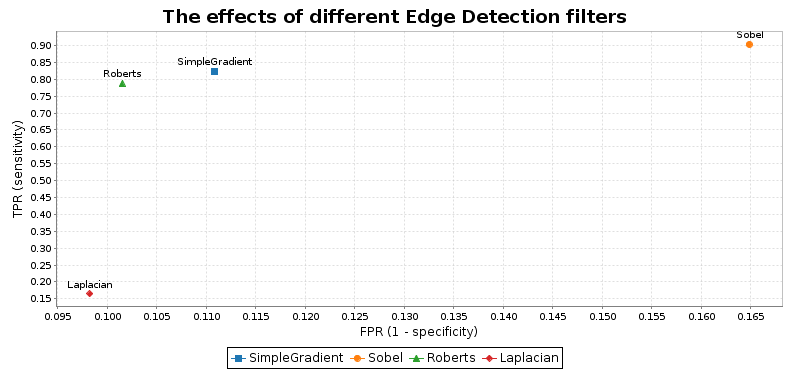
\includegraphics[scale=0.5]{graphs/1-edge_detect_all.png}
\caption{ROC analysis on 10905 JL, using Gaussian for noise removal}
\label{fig:edgedetectors}
\end{figure}

The use of Laplacian yielded some interesting results. Although it had very precise lines, we found that it tended to perceive cells smaller than the samples. This is why it had worse results in ROC analysis, as ROC analysis doesn’t take into account small transformations. This a major flaw of ROC, and perhaps different methods of verification can be used to evaluate edge detection systems.

With Laplacian, we were able to combine it with Gaussian by convolving the matrices with each other. This lead to the same result, but cut the operation time by more than a factor of 3, from 823ms to 226ms. This is due to only having to perform one large convolution with the combination of the filters, rather than both separately.
\subsubsection*{Final Thresholding}

\begin{figure}[h]
\centering
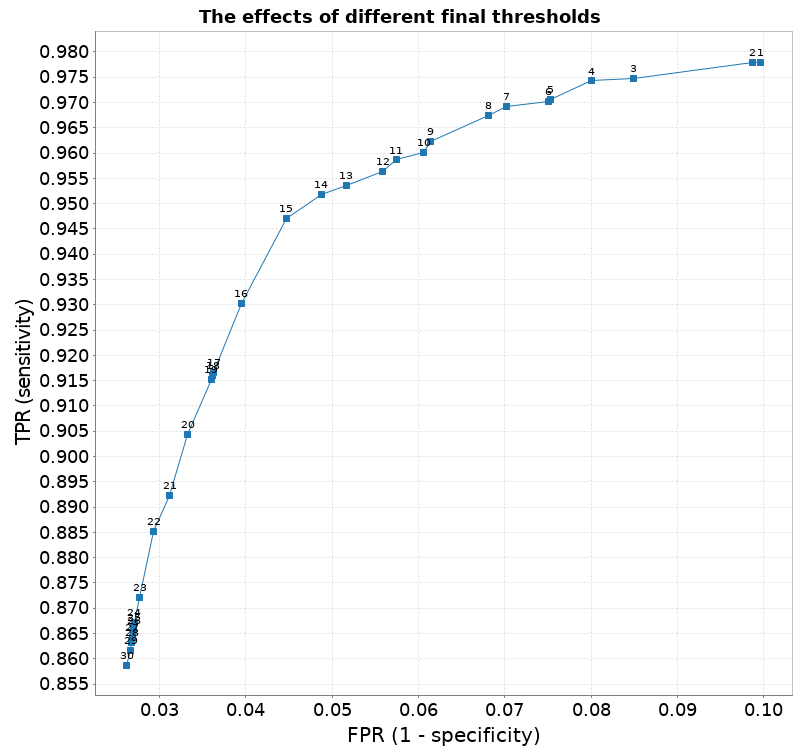
\includegraphics[width=0.75\textwidth]{graphs/threshold_example}
\caption{ROC analysis of final threshold variation}
\label{fig:finalthreshold}
\end{figure}

When applying the final threshold, perfect values vary on a case-to-case basis. ROC analysis was especially useful here - plotting points for regular intervals of thresholds allowed us to see exactly what the ideal value is. For example, if we vary the threshold on a combination of noise removal and edge detection, we get the curve illustrated in figure~\ref{fig:finalthreshold}.

This allows us to see that the ideal threshold is around 15. We can also calculate the best threshold by determining the point with the smallest distance from the optimal point of (0, 1). As these values vary, it is very difficult to decide a “best” general value, and instead needs recalculations for every case.



%\vspace{16mm}


\section*{Conclusion}
One of the interesting conclusions that can be drawn from this is the balancing act of noise removal. Too little, and insignificant pixels have an impact on the end result, and too much leads to thicker edges. There are ways of dealing with thicker edges, such as Canny, but in general trying to have as little blurring while keeping away background noise is good practice.

For edge detection, we found that the Roberts filter lead to much thinner edges than Sobel. This could be due to it’s 2x2 filter, rather than 3x3. This means that pixels have to be closer to the edge to be impacted on, meaning less pixels are marked as edges, therefore there are thinner lines.

And finally, with thresholding at the end of these operations, it varies on a case-to-case basis (as mentioned before), and ROC analysis is a great tool for this.
Edge detection isn’t a “one size fits all” solution. Operations have to be tweaked at every stage in the process - even in this case with three similar images, the thresholds have varying optimum values. Finding the best operations can be done manually, by brute force, or even with machine learning.


%\end{multicols}

\end{document}